% Options for packages loaded elsewhere
\PassOptionsToPackage{unicode}{hyperref}
\PassOptionsToPackage{hyphens}{url}
\PassOptionsToPackage{dvipsnames,svgnames,x11names}{xcolor}
%
\documentclass[
]{article}

\usepackage{amsmath,amssymb}
\usepackage{iftex}
\ifPDFTeX
  \usepackage[T1]{fontenc}
  \usepackage[utf8]{inputenc}
  \usepackage{textcomp} % provide euro and other symbols
\else % if luatex or xetex
  \usepackage{unicode-math}
  \defaultfontfeatures{Scale=MatchLowercase}
  \defaultfontfeatures[\rmfamily]{Ligatures=TeX,Scale=1}
\fi
\usepackage[]{times}
\ifPDFTeX\else  
    % xetex/luatex font selection
\fi
% Use upquote if available, for straight quotes in verbatim environments
\IfFileExists{upquote.sty}{\usepackage{upquote}}{}
\IfFileExists{microtype.sty}{% use microtype if available
  \usepackage[]{microtype}
  \UseMicrotypeSet[protrusion]{basicmath} % disable protrusion for tt fonts
}{}
\makeatletter
\@ifundefined{KOMAClassName}{% if non-KOMA class
  \IfFileExists{parskip.sty}{%
    \usepackage{parskip}
  }{% else
    \setlength{\parindent}{0pt}
    \setlength{\parskip}{6pt plus 2pt minus 1pt}}
}{% if KOMA class
  \KOMAoptions{parskip=half}}
\makeatother
\usepackage{xcolor}
\setlength{\emergencystretch}{3em} % prevent overfull lines
\setcounter{secnumdepth}{2}
% Make \paragraph and \subparagraph free-standing
\ifx\paragraph\undefined\else
  \let\oldparagraph\paragraph
  \renewcommand{\paragraph}[1]{\oldparagraph{#1}\mbox{}}
\fi
\ifx\subparagraph\undefined\else
  \let\oldsubparagraph\subparagraph
  \renewcommand{\subparagraph}[1]{\oldsubparagraph{#1}\mbox{}}
\fi


\providecommand{\tightlist}{%
  \setlength{\itemsep}{0pt}\setlength{\parskip}{0pt}}\usepackage{longtable,booktabs,array}
\usepackage{calc} % for calculating minipage widths
% Correct order of tables after \paragraph or \subparagraph
\usepackage{etoolbox}
\makeatletter
\patchcmd\longtable{\par}{\if@noskipsec\mbox{}\fi\par}{}{}
\makeatother
% Allow footnotes in longtable head/foot
\IfFileExists{footnotehyper.sty}{\usepackage{footnotehyper}}{\usepackage{footnote}}
\makesavenoteenv{longtable}
\usepackage{graphicx}
\makeatletter
\def\maxwidth{\ifdim\Gin@nat@width>\linewidth\linewidth\else\Gin@nat@width\fi}
\def\maxheight{\ifdim\Gin@nat@height>\textheight\textheight\else\Gin@nat@height\fi}
\makeatother
% Scale images if necessary, so that they will not overflow the page
% margins by default, and it is still possible to overwrite the defaults
% using explicit options in \includegraphics[width, height, ...]{}
\setkeys{Gin}{width=\maxwidth,height=\maxheight,keepaspectratio}
% Set default figure placement to htbp
\makeatletter
\def\fps@figure{htbp}
\makeatother
% definitions for citeproc citations
\NewDocumentCommand\citeproctext{}{}
\NewDocumentCommand\citeproc{mm}{%
  \begingroup\def\citeproctext{#2}\cite{#1}\endgroup}
\makeatletter
 % allow citations to break across lines
 \let\@cite@ofmt\@firstofone
 % avoid brackets around text for \cite:
 \def\@biblabel#1{}
 \def\@cite#1#2{{#1\if@tempswa , #2\fi}}
\makeatother
\newlength{\cslhangindent}
\setlength{\cslhangindent}{1.5em}
\newlength{\csllabelwidth}
\setlength{\csllabelwidth}{3em}
\newenvironment{CSLReferences}[2] % #1 hanging-indent, #2 entry-spacing
 {\begin{list}{}{%
  \setlength{\itemindent}{0pt}
  \setlength{\leftmargin}{0pt}
  \setlength{\parsep}{0pt}
  % turn on hanging indent if param 1 is 1
  \ifodd #1
   \setlength{\leftmargin}{\cslhangindent}
   \setlength{\itemindent}{-1\cslhangindent}
  \fi
  % set entry spacing
  \setlength{\itemsep}{#2\baselineskip}}}
 {\end{list}}
\usepackage{calc}
\newcommand{\CSLBlock}[1]{\hfill\break#1\hfill\break}
\newcommand{\CSLLeftMargin}[1]{\parbox[t]{\csllabelwidth}{\strut#1\strut}}
\newcommand{\CSLRightInline}[1]{\parbox[t]{\linewidth - \csllabelwidth}{\strut#1\strut}}
\newcommand{\CSLIndent}[1]{\hspace{\cslhangindent}#1}

% Place figures and tables exactly where they were called
\usepackage{float}
\floatplacement{figure}{H}
\floatplacement{table}{H}

% Recommended by the modelsummary package
\usepackage{booktabs}
\usepackage{siunitx}
\newcolumntype{d}{S[input-symbols = ()]}

% Add affiliations (title.tex needs to be called under template-partials)
\usepackage[noblocks]{authblk}
\renewcommand*{\Authsep}{, }
\renewcommand*{\Authand}{, }
\renewcommand*{\Authands}{, }
\renewcommand\Affilfont{\small}

% Add line numbers
\usepackage{lineno}
\linenumbers
\usepackage{booktabs}
\usepackage{longtable}
\usepackage{array}
\usepackage{multirow}
\usepackage{wrapfig}
\usepackage{float}
\usepackage{colortbl}
\usepackage{pdflscape}
\usepackage{tabu}
\usepackage{threeparttable}
\usepackage{threeparttablex}
\usepackage[normalem]{ulem}
\usepackage{makecell}
\usepackage{xcolor}
\usepackage{siunitx}

  \newcolumntype{d}{S[
    input-open-uncertainty=,
    input-close-uncertainty=,
    parse-numbers = false,
    table-align-text-pre=false,
    table-align-text-post=false
  ]}
  
\makeatletter
\@ifpackageloaded{caption}{}{\usepackage{caption}}
\AtBeginDocument{%
\ifdefined\contentsname
  \renewcommand*\contentsname{Table of contents}
\else
  \newcommand\contentsname{Table of contents}
\fi
\ifdefined\listfigurename
  \renewcommand*\listfigurename{List of Figures}
\else
  \newcommand\listfigurename{List of Figures}
\fi
\ifdefined\listtablename
  \renewcommand*\listtablename{List of Tables}
\else
  \newcommand\listtablename{List of Tables}
\fi
\ifdefined\figurename
  \renewcommand*\figurename{Figure}
\else
  \newcommand\figurename{Figure}
\fi
\ifdefined\tablename
  \renewcommand*\tablename{Table}
\else
  \newcommand\tablename{Table}
\fi
}
\@ifpackageloaded{float}{}{\usepackage{float}}
\floatstyle{ruled}
\@ifundefined{c@chapter}{\newfloat{codelisting}{h}{lop}}{\newfloat{codelisting}{h}{lop}[chapter]}
\floatname{codelisting}{Listing}
\newcommand*\listoflistings{\listof{codelisting}{List of Listings}}
\makeatother
\makeatletter
\@ifpackageloaded{caption}{}{\usepackage{caption}}
\@ifpackageloaded{subcaption}{}{\usepackage{subcaption}}
\makeatother
\makeatletter
\makeatother
\ifLuaTeX
  \usepackage{selnolig}  % disable illegal ligatures
\fi
\IfFileExists{bookmark.sty}{\usepackage{bookmark}}{\usepackage{hyperref}}
\IfFileExists{xurl.sty}{\usepackage{xurl}}{} % add URL line breaks if available
\urlstyle{same} % disable monospaced font for URLs
\hypersetup{
  pdftitle={Paper Title},
  pdfauthor={John Doe; Jeanne Doe},
  pdfkeywords={Repoducible, R},
  colorlinks=true,
  linkcolor={blue},
  filecolor={Maroon},
  citecolor={red},
  urlcolor={Blue},
  pdfcreator={LaTeX via pandoc}}

\title{Paper Title}


  \author{John Doe}
            \affil{%
                  Deadliest University
              }
        \author{Jeanne Doe}
            \affil{%
                  Random University
              }
      
\date{2023-09-29}
\begin{document}
\maketitle
\begin{abstract}
Abstract: this research is so awesome that you cannot reject this paper.
\end{abstract}
\newpage

\section{Introduction}\label{introduction}

The issue this article addresses is \textbf{super} \emph{important}!

\begin{itemize}
\item
  \textbf{author names and year}:
  (\citeproc{ref-schlenker2009nonlinear}{1}) examined \ldots.
\item
  \textbf{author names and year in parentheses}:
  (\citeproc{ref-schlenker2009nonlinear}{1})
\item
  \textbf{multiple citations in parentheses}:
  (\citeproc{ref-schlenker2009nonlinear}{1},
  \citeproc{ref-mas1995microeconomic}{2})
\item
  \textbf{only year in parentheses}:
  (\citeproc{ref-schlenker2009nonlinear}{1})
\end{itemize}

\newpage

\section{Materials and Methods}\label{materials-and-methods}

\subsection{Data}\label{data}

The number of observations are 598 and 1376 for Zones 2 and 3,
respectively.

Table Table~\ref{tbl-summary-statistics} presents summary statistics by
zone.

\subsection{Statistical Model}\label{statistical-model}

See equation \ref{eq-equation} and \ref{eq-align} for the statistical
models we use.

\begin{equation}
y = \beta_0 + \beta_1 x + \varepsilon \label{eq-equation}
\end{equation}

\begin{align}
Y_z & = f_z(S) + g_z(N) + h_z(X,Y) + \varepsilon_z \notag \\
& = \sum_{i=1}^k \phi_k(S) + g_z(N) + h_z(X,Y) + \varepsilon_z \label{eq-align}
\end{align}

Our target coefficient is \(\beta_1\) (in-line math).

\begin{equation}\phantomsection\label{eq-simple}{
y = \beta_0 + \beta_1 x + \varepsilon 
}\end{equation}

Equation Equation~\ref{eq-simple} is correctly cross-referenced.

\section{Results and Discussions}\label{results-and-discussions}

Table Table~\ref{tbl-reg-table} presents the regression results.

Figure Figure~\ref{fig-yield-dist} presents the distribution of yields
by zone.

\section{Conclusions}\label{conclusions}

bluh bluh\footnote{This is a footnote}, another bluh bluh\footnote{This
  is the second footnote}

\section{Figures}\label{figures}

I like Figure~\ref{fig-yield-dist} a lot.

\begin{figure}

\centering{

\includegraphics[width=0.8\textwidth,height=0.8\textheight]{index_files/figure-pdf/fig-yield-dist-1.pdf}

}

\caption{\label{fig-yield-dist}The Distribution of Yield by Zone}

\end{figure}%

Figure~\ref{fig-imported-plot} was imported.

When width or height is not specified, the original dimension of the
saved figure is respected.

\begin{figure}

\centering{

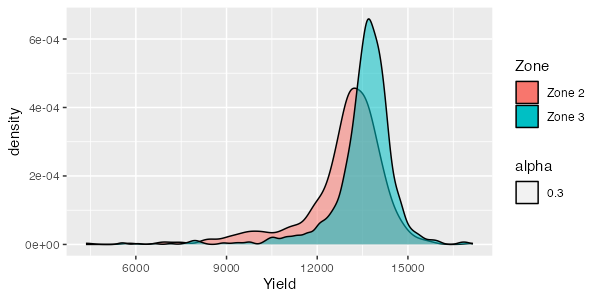
\includegraphics{g_plot_external.pdf}

}

\caption{\label{fig-imported-plot}Imported Plot}

\end{figure}%

\section{Tables}\label{tables}

\subsection{\texorpdfstring{Use the \texttt{modelsummary} package to
create regression results
tables}{Use the modelsummary package to create regression results tables}}\label{use-the-modelsummary-package-to-create-regression-results-tables}

\begin{table}

\caption{\label{tbl-reg-table}Regression results table by the
modelsummary function}

\centering{

\begin{table}
\centering
\begin{tabular}[t]{lccc}
\toprule
  & (1) & (2) & (3)\\
\midrule
(Intercept) & \num{36.908} & \num{38.752} & \num{38.752}\\
 & (\num{2.191}) & (\num{1.787}) & (\num{1.857})\\
hp & \num{-0.019} & \num{-0.018} & \num{-0.018}\\
 & (\num{0.015}) & (\num{0.012}) & (\num{0.009})\\
cyl & \num{-2.265} & \num{-0.942} & \num{-0.942}\\
 & (\num{0.576}) & (\num{0.551}) & (\num{0.799})\\
wt &  & \num{-3.167} & \num{-3.167}\\
 &  & (\num{0.741}) & (\num{1.691})\\
\midrule
Num.Obs. & \num{32} & \num{32} & \num{32}\\
R2 & \num{0.741} & \num{0.843} & \num{0.843}\\
RMSE & \num{3.02} & \num{2.35} & \num{2.35}\\
Std.Errors & IID & IID & by: vs\\
\bottomrule
\end{tabular}
\end{table}

}

\end{table}%

Table Table~\ref{tbl-reg-table} shows the regression results.

\begin{table}

\caption{\label{tbl-reg-table-mod-with-kE}Regression results table by
the modelsummary function}

\centering{

\begin{table}
\centering
\begin{tabular}[t]{lccc}
\toprule
\multicolumn{1}{c}{ } & \multicolumn{2}{c}{Model (se not clustered) } & \multicolumn{1}{c}{Model (se clustered)} \\
\cmidrule(l{3pt}r{3pt}){2-3} \cmidrule(l{3pt}r{3pt}){4-4}
  & (1) & (2) & (3)\\
\midrule
(Intercept) & \num{36.908}*** & \num{38.752}*** & \num{38.752}*\\
 & (\num{2.191}) & (\num{1.787}) & (\num{1.857})\\
hp & \num{-0.019} & \num{-0.018} & \num{-0.018}\\
 & (\num{0.015}) & (\num{0.012}) & (\num{0.009})\\
cyl & \num{-2.265}*** & \num{-0.942}+ & \num{-0.942}\\
 & (\num{0.576}) & (\num{0.551}) & (\num{0.799})\\
wt &  & \num{-3.167}*** & \num{-3.167}\\
 &  & (\num{0.741}) & (\num{1.691})\\
\midrule
Num.Obs. & \num{32} & \num{32} & \num{32}\\
R2 & \num{0.741} & \num{0.843} & \num{0.843}\\
RMSE & \num{3.02} & \num{2.35} & \num{2.35}\\
Std.Errors & IID & IID & by: vs\\
\bottomrule
\multicolumn{4}{l}{\rule{0pt}{1em}+ p $<$ 0.1, * p $<$ 0.05, ** p $<$ 0.01, *** p $<$ 0.001}\\
\end{tabular}
\end{table}

}

\end{table}%

Table~\ref{tbl-reg-table-mod-with-kE} shows the regression results
created by modelsummary(), which is then modified by the kableExtra
package (additional row added at the top).

\begin{table}

\caption{\label{tbl-summary-statistics}Summary Statistics by Zone}

\centering{

\begin{table}
\centering
\begin{tabular}[t]{llrrrrr}
\toprule
Zone &   & get\_N & Mean & SD & Min & Max\\
\midrule
Zone 2 & Yield (kg/ha)` <- Yield & 598 & \num{12876.63} & \num{1445.67} & \num{4349.84} & \num{17150.77}\\
 & Nitrogen Rate (kg/ha)` <- aa\_n & 598 & \num{117.82} & \num{14.73} & \num{88.94} & \num{145.57}\\
 & Seed Rate (1000/ha)` <- aa\_s & 598 & \num{84.01} & \num{6.86} & \num{69.17} & \num{98.61}\\
Zone 3 & Yield (kg/ha)` <- Yield & 1376 & \num{13530.20} & \num{1093.98} & \num{5539.50} & \num{16966.78}\\
 & Nitrogen Rate (kg/ha)` <- aa\_n & 1376 & \num{118.20} & \num{14.61} & \num{88.84} & \num{143.75}\\
 & Seed Rate (1000/ha)` <- aa\_s & 1376 & \num{87.20} & \num{7.03} & \num{69.58} & \num{98.82}\\
\bottomrule
\end{tabular}
\end{table}

}

\end{table}%

Table Table~\ref{tbl-summary-statistics} shows summary statistics.

\newpage

\section{Appendix}\label{appendix}

itemized list (this does not work) + item 1 + item 2 + item 3

itemized list

\begin{itemize}
\tightlist
\item
  item 1
\item
  item 2
\item
  item 3
\end{itemize}

nested list

\begin{itemize}
\tightlist
\item
  item 1

  \begin{itemize}
  \tightlist
  \item
    item 1.1
  \item
    item 1.2
  \end{itemize}
\item
  item 2
\item
  item 3
\end{itemize}

enumerated list

\begin{enumerate}
\def\labelenumi{\arabic{enumi}.}
\tightlist
\item
  item 1
\item
  item 2
\item
  item 3
\end{enumerate}

\newpage

\section*{References}\label{references}
\addcontentsline{toc}{section}{References}

\phantomsection\label{refs}
\begin{CSLReferences}{0}{1}
\bibitem[\citeproctext]{ref-schlenker2009nonlinear}
\CSLLeftMargin{1. }%
\CSLRightInline{W. Schlenker, M. J. Roberts, Nonlinear temperature
effects indicate severe damages to US crop yields under climate change.
\emph{Proceedings of the National Academy of sciences} \textbf{106},
15594--15598 (2009).}

\bibitem[\citeproctext]{ref-mas1995microeconomic}
\CSLLeftMargin{2. }%
\CSLRightInline{A. Mas-Colell, M. D. Whinston, J. R. Green, \emph{et
al.}, \emph{Microeconomic theory} (Oxford university press New York,
1995).}

\end{CSLReferences}



\end{document}
